\documentclass[10pt,a4paper]{article}

\usepackage[utf8]{inputenc}
\usepackage{hyperref}
\usepackage{siunitx}
\usepackage{circuitikz}
\usepackage{amsmath}
\usepackage{amsfonts}
\usepackage{amssymb}
\usepackage{float}
\usepackage{graphicx}
\usepackage{wrapfig}
\usepackage{caption}
\usepackage{subcaption}
\newcommand{\uuline}[1]{\underline{\underline{#1}}}

\author{\textbf{Students: }Robin Dorstijn, Moritz Epping \\ \textbf{Tutor: }Jakob Kaiser}
\title{Lab Report FP09: Neuromorphic computing}
\date{February 2021}

\begin{document}
\maketitle
\clearpage
\tableofcontents

\clearpage
\begin{abstract}
    This paper presents a review of the SPIKEY chip for neuromorphic
    computing.  After a theoretical framework outlining the requirements
    for a simple neuromorphic computing device has been given, this
    specific hardware realization will be examined under these considerations.
    It will be shown that the SPIKEY chip exhibits all of the bas`
\end{abstract}

\section{Theoretical Foundations}
\subsection{General background}
\subsubsection{Motivation}
Brains and computers often are compared because of their shared purpose:
decision making, though they have irreconcilable differences in architecture.
Modern computers function on the basis of the van Neumann
architecture\cite{von-Neumann}, which separates the control unit from the memory
and the computation unit. Though this simplifies the structure of the computer
and makes it modular, it however does create a clear bottleneck at the
communication layer, commonly known as the von Neumann bottleneck. This creates
an energy inefficiency that is unacceptable for biological systems like that of
humans, who spend around 20\% of their total energy uptake on the
brain\cite{metabolic-rates}.  This most likely has provided significant
evolutionary pressure for hominids to optimize metabolic resource
usage\cite{seymour2016fossil}. For this reason a new architecture for computers
has been suggested: neuromorphic\footnote{``Neuro'' as in brain, ``-morphic'' as
in having the shape of, forming ``having the shape of a brain''.} computing.
Besides more efficient energy usage,  the scientific interest in neuromorphic
computing is also grounded in the idea of trying to understand the human brain
by rebuilding it artificially.

\subsubsection{Signal processing in the brain}
Neurons are the basic computational components of the brain, transmitting and
morphing signals. Each neuron receives signals from others at the dendrites,
which shift the electric potential at the membrane of the cell at the site of
the synapse\footnote{Synapse: the connection point of two dendrites where the
axon of one meets the dendrite of the other.}. Once a critical amount of
potential has been built up, an ion wave crossing the entire membrane of the
neuron, reaching it's axon, allowing it to pass the signal on to other neurons.

The potential at the neuron membrane as a function of time has three main
domains: first there is the rest voltage, where the membrane potential is at its
natural equilibrium, which gets perturbed by synaptic input. Pumps in the cell
membrane cause the potential to return to an equilibrium. If sufficient signals
arrive at the neuron with a run away effect is induced, where the potential
exponentially increases, until it hits a maximum, leading into a third phase:
hyperpolarisation. The cell so quickly returns to its natural potential that it
`overshoots' and is temporarily negatively charged with respect to the natural
potential, making it less sensitive to input for a short time after having
created the peak.

\begin{figure}[ht]
    \centering
    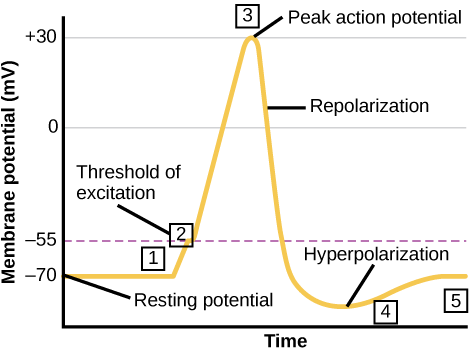
\includegraphics[width=\textwidth]{figures/action-potential.png}
    \caption{Formation of an action potential. Source:  \url{https://courses.lumenlearning.com/boundless-biology/chapter/how-neurons-communicate/}}
    \label{fig:action-potential}
\end{figure}

\subsubsection{The LIF model}
In order to emulate the behaviour electronically, a leaky integrate and fire
(LIF) model is used. A single neuron is represented by an electronic circuit
like the one in figure \ref{fig:circuit}. A constant ``leak'' voltage present on
the membrane, representing the biological rest potential of the membrane
potential.  The neuron, represented as a capacitor with capacitance $C_m$ is
charged and decharged by the input of other neurons. With constant excitatory
(facilitating spikes) and inhibitory (suppressing spikes) potential,  all
dynamics are encoded in the time-dependent conductances $g_i(t),  g_x(t)$. A
spike coming from either of these two synapse types is implemented by
temporarily increasing the corresponding conductance. When the threshold
voltage $V_\text{thres}$,  is reached, the amplifier functioning as a comparator
in this setting,  sends out a $V_{CC}$ signal to a digital unit that processes
that the neuron has fired and is responsible for closing the switch that keeps
the ``membrane potential'' $V_m$ at some $V_\text{reset}$ for the refractory
period. This time is meant to mimic the period during which the voltage at the
membrane increases non-linearly and therefore loses its sensitivity to input.
The digital processing unit is also responsible for sending the signal (in terms
of a uniform spike; ``All-or-nothing reponse'') to the neurons that the are
connected to the one that just fired.  The synapses then transform this voltage
spike into an excitatory or inhibitory input for the other neurons.

\begin{figure}[ht]
    \centering
    \begin{circuitikz}[scale = .6, transform shape]
        \draw (0, 0)    to node[midway, above]{$V_m$} (8.5, 0) node[op amp, anchor=+](A1){}; % main line
        \draw (A1.out)  to[short, l=$V_\text{out}$, -o] ++(1, 0);
        \draw (7, 1)    node[left, above] {$V_\text{thres}$} to[short, *-] (A1.-);
        \draw (0, 0)    to[vR, l=$g_{i, j}$, *-] ++(0, -2)
                        to[battery1, l=$E_{i, j}$] ++(0, -1) node[ground] {} ++(0, -1);
        \draw (2, 0)    to[vR, l=$g_{x, j}$, *-] ++(0, -2)
                        to[battery1, l=$E_{x, j}$] ++(0, -1) node[ground] {} ++(0, -1);
        \draw (4, 0)    to[vR, l=$g_l$, *-] ++(0, -2)
                        to[battery1, l=$E_l$] ++(0, -1) node[ground] {} ++(0, -1);
        \draw (6, 0)    to[C, l=$C_m$] (6, -2)
                        node[ground] {} (6, -2);
        \draw (7.5, -2) node[anchor=north] {$V_\text{reset}$}
                        to[short, o-] (7.5, -1)
                        to[normal open switch, -*] (7.5, 0);
        \draw [densely dashed]
              (3.3, -4) --++(0, 4.6)
                        --++(5, 0)
                        --++(0, -4.6)
                        --++(-5, 0);
    \end{circuitikz}
    \caption{Circuit of a single neuron in a LIF chip.}
    \label{fig:circuit}
\end{figure}


\begin{figure}[ht]
    \centering
    \begin{circuitikz}[scale = .6, transform shape]
        \draw (4, 0)    to node[midway, above]{$V_m$} (8.5, 0) node[op amp, anchor=+](A1){}; % main line
        \draw (A1.out)  to[short, l=$V_\text{out}$, -o] ++(1, 0);
        \draw (7, 1)    node[left, above] {$V_\text{thres}$} to[short, *-] (A1.-);
        \draw (4, 0)    to[vR, l=$g_i$, *-] (4, -2)
                        to[battery1, l=$E_g$] (4, -3) node[ground] {} (4, -4);
        \draw (6, 0)    to[C, l=$C_m$] (6, -2)
                        node[ground] {} (6, -2);
        \draw (8, -3)   to[short, l_=$V_\text{reset}$, o-] (8, -1)
                        to[short, o-] (7.5, -1)
                        to[normal open switch, -*] (7.5, 0);
    \end{circuitikz}
    \caption{Circuit of a single neuron in a LIF chip.}
    \label{fig:circuit-simplified}
\end{figure}


\subsection{Investigating A Single Neuron}

\subsection{Calibrating Neuron Parameters}
In the case of a single unconnected neuron the membrane potential can be
understood with application of the Kirchoff formula to the circuit in figure
\ref{fig:circuit-simplified}.
\[
    C_m \frac{dV_m}{dt} = g_l(E_l - V_m)
\]
This is a ordinary first order differential equation and has the
solution
\begin{equation}
    V_m(t) = A \exp(\frac{-g_l}{C_m}t) - E_l
    \label{eq:diff-eq-sol}
\end{equation}
where $A$ is given by the initial condition:
\[
    A = V_m(0) - E_l.
\]

In order to set a neuron to fire at a regular frequency $\tau$, we have to take
into account that $V_m$ will be reset to $V_\text{reset}$ when it hits
$V_\text{thres}$. Equation \eqref{eq:diff-eq-sol} can be rephrased in terms of
$t$.
\begin{equation}
    \tau = -\ln(\frac{V_\text{thres} - E_l}{V_\text{reset} - E_l})
    \frac{C_m}{g_l}
    \label{eq:tau}
\end{equation}

The characteristic time constant $\tau_m$ of the system can be found by setting
$V_\text{thres}$ as a function of $E_l$ and $V_\text{reset}$.
\[
    V_\text{thres} = E_l - (E_l - V_\text{reset})\exp(-1)
\]
The resulting $\tau_m$ is then only dependent on $C_m$ and $g_l$:
\begin{align*}
    \tau_m &= -\ln(\frac{E_l - (E_l - (E_l - V_\text{reset})\exp(-1))}{V_\text{reset} - E_l}) \frac{C_m}{g_l}\\
           &= -\ln(\frac{(E_l - V_\text{reset})\exp(-1))}{V_\text{reset} - E_l})\frac{C_m}{g_l} \\
           &= \frac{C_m}{g_l}
\end{align*}
This time constant does not take into account the refractory period which should
add a fixed contribution. This describes a good theory of the firing  neuron,
however in reality there are some serious production artifacts that require
calibration.

\subsection{A Single Neuron with Synaptic Input}

\subsection{Short Term Plasticity}

\subsection{Feed-Forward Networks}
One of the simplest neural networks one can consider is the feed-forward network
in which every neuron is arranged so that it passes on the signal it receives to
the next. In nature, a single neuron firing has relatively little meaning until
it is put in a larger context. Most of these contexts can be simplified by
viewing them as `superpositions' feed forward networks. It is however important
to consider that in nature robustness and redundancy is highly favored in
critical systems. The function of a feed-forward network can be shutdown
entirely if one neuron fails for whatever reason. Hence the concept of
populations is introduced, these are groups of neurons that perform the same
logical operations\footnote{That is to say, they are all either inhibitory or
excitatory neurons and share the same characteristics. Variations may be
introduced from a normal distribution. Note that this definition matches well
with pyNN, but might not be used identically in all literature.} This is
visualised in figure \ref{fig:feed-forward}.

\begin{wrapfigure}{r}{0.5\textwidth}
    \centering
    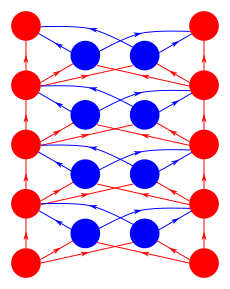
\includegraphics[width=.3\textwidth]{figures/feedforward-real.png}
    \caption{Feed forward network with length 4 and population size 2. Two input
        neurons are drawn additionally. Inhibitory neurons and connections are drawn
        in red, inhibitory ones in blue.}
    \label{fig:feed-forward}
\end{wrapfigure}

In this experiment, connection weights also become relevant for the first time.
Any synaptic connection is assigned a weight, this weight affects the
membrane potential increase that a signal transfer induces. The importance of
this variable is crucial for networks as it nearly completely describes the
behaviour of a network.

A synfire\footnote{Synfire: a type of feed forward network that is a simple
    chain of single excitatory neurons coupled in succession. Alternative
    structures are described as feed forward networks as well, for example
    situations where each excitatory neuron connects to at least two other
    neurons in the next layer.  These structures are more complicated and out of
the scope of this report.} feed-forward network is described by the population
number, the chain length (see figure \ref{fig:feed-forward}) and the several
weights of the following type connections:

\begin{itemize}
    \item From the initial excitatory neuron to the first excitatory member of the
        chain. (ex0 $\rightarrow$ ex)
    \item From the initial excitatory neuron to the first inhibitory member of the
        chain. (ex0 $\rightarrow$ inh)
    \item From an excitatory neuron in the chain to the next excitatory neuron.
        (ex $\rightarrow$ ex)
    \item From an excitatory neuron in the chain to the next inhibitory neuron.
        (ex $\rightarrow$ inh)
    \item From an inhibitory neuron in the chain to the next excitatory neuron.
        (inh $\rightarrow$ ex)
\end{itemize}

\subsection{Recurrent Networks}

\subsection{A Simple Computation - XOR}
A very common binary operation that is particularly non-linear is the XOR
operation\cite{horowitz_hill_2020}. A trivial solution for this problem was
found (see figure \ref{fig:XOR-suggested}) and dismissed thanks to its probable
fragility. Instead the institute provided a different network architecture that
has significant benefits over the suggested one: it is much more robust to what
is called referred to with `width' in section \ref{sec:feed-forward}. The
inhibitory neurons that are operating in a recurrent fashion prevent leaking
voltage from causing the any excitatory neuron in the network to fire out of
line. This is especially important in an XOR gate, as the chance that noise
would `cancel out' is negligible.
\begin{table}[ht]
    \centering
    \begin{tabular}{c | c | c}
        A & B & Q \\ \hline
        0 & 0 & 0 \\
        0 & 1 & 1 \\
        1 & 0 & 1 \\
        1 & 1 & 0
    \end{tabular}
    \caption{Truth table of the XOR gate. For more information see:
    \cite{horowitz_hill_2020}}
    \label{tab:XOR}
\end{table}

A simple solution for this problem is presented in figure
\ref{fig:XOR-suggested}, however this was not used, as the institute provided a
different network architecture that has significant benefits over the suggested
one: it is much more robust to what is called referred to with `width' in
section \ref{sec:feed-forward}. The inhibitory neurons that are operating in a
recurrent fashion prevent leaking voltage from causing the any excitatory neuron
in the network to fire out of line. This is especially important in an XOR gate,
as the chance that noise would `cancel out' is negligible.

\begin{figure}
    \centering
    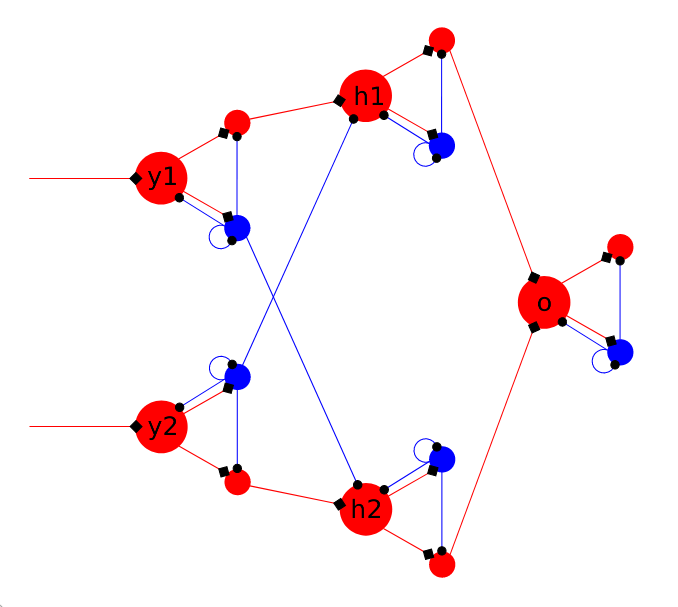
\includegraphics[width=\textwidth]{figures/XOR-used.png}
    \caption{Network that was used to test the ability of neurons to perform
        logical operations. Functions as an XOR gate.}
    \label{fig:XOR-used}
\end{figure}

\begin{wrapfigure}{r}{0.5\textwidth}
    \centering
    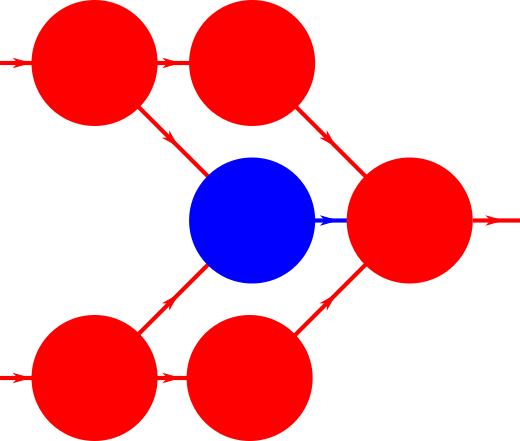
\includegraphics[width=.3\textwidth]{figures/XOR-suggested.png}
    \caption{Suggestion for a network that behaves like an XOR gate. Note that
        the inhibitory weight has to be strong, so that it can inhibit the output
        from signalling, even when it receives an input from both sides.}
    \label{fig:XOR-suggested}
\end{wrapfigure}

\section{Experimental Procedure}

\subsection{Investigating A Single Neuron}
To assess the reliability of the spikey chip, it is first necessary to investigate
the most simple configuration. This consists of a single neuron without any
input.  As described in section 1.3,  the circuit then simplifies significantly.
The chip can be configured in this setup by setting the conductances
corresponding to other inputs to zero.  \par
By setting the leakage potential above the threshold potential, we can bring
the neuron into a constant firing regime despite no other synaptic input.
Values of $E_l = -50$mV and $V_{thres} = -55$mV.  The firing rate was
measured to equal $t_{fir} = (16.10\pm0.11)$ms.  According to the circuit
diagram,  the operation of the spikey chip in this setup corresponds to
charging a capacitor with a current given by $I(t) = g_l(t)E_l$.  This
characteristic voltage behaviour of charging a capacitor can be seen
in \ref{fig:membranes_ex1}.  When increasing the leakage conductance $g_l$ we
could observe shorter spike times.  This agrees well with our theoretical
understanding of the model since we essentially charge the current with a
stronger current,  thus reaching the firing-inducing threshold voltage sooner.
\begin{figure}[ht]
    \centering
    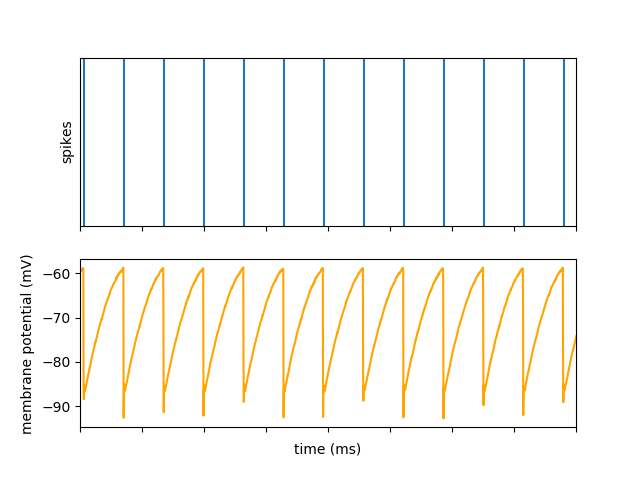
\includegraphics[width=\textwidth]{figures/fp_task1_1membrane.png}
    \caption{Voltage over a single neuron with leakage potential over threshold potential}
    \label{fig:membranes_ex1}
\end{figure}


\subsection{Calibrating Neuron Parameters}
On the SPIKEY chip 4 neurons were isolated programmatically and given the same
parameters:
\begin{itemize}
    \item $V_\text{reset}$: \SI{-80.0}{\milli\volt}
    \item $V_\text{thresh}$: \SI{-55.0}{\milli\volt}
    \item $E_\text{leak}$: \SI{-50.0}{\milli\volt}
    \item $g_\text{leak}$:  \SI{20.0}{\nano\siemens}
\end{itemize}
This however resulted in wildly differing frequencies. In order to compensate
for this $g_l$ was adjusted individually for all of the membranes so that they
were all correct within their respective standard deviation:
\SI{20.1}{\milli\volt}, \SI{55.0}{\milli\volt}, \SI{60.0}{\milli\volt},
\SI{20.5}{\milli\volt}.

\begin{figure}[ht]
    \centering
    \begin{subfigure}[t]{\textwidth}
        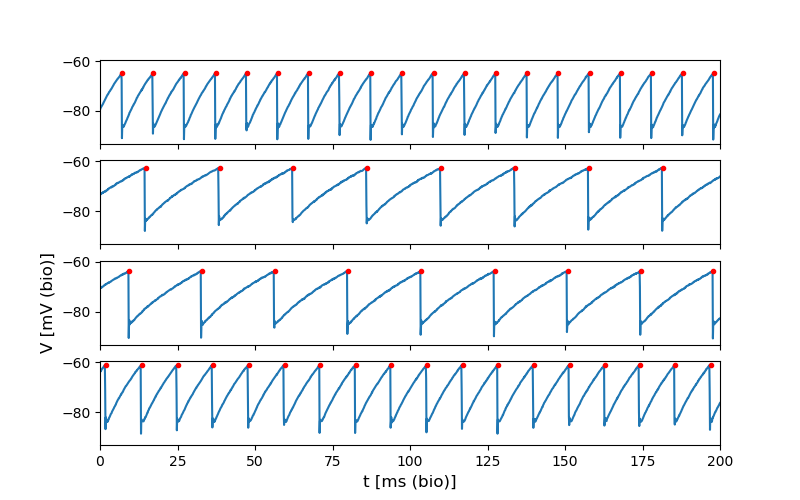
\includegraphics[width=\textwidth]{figures/4membranes.png}
        \caption{Uncalibrated membranes}
    \end{subfigure}
    \begin{subfigure}[b]{\textwidth}
        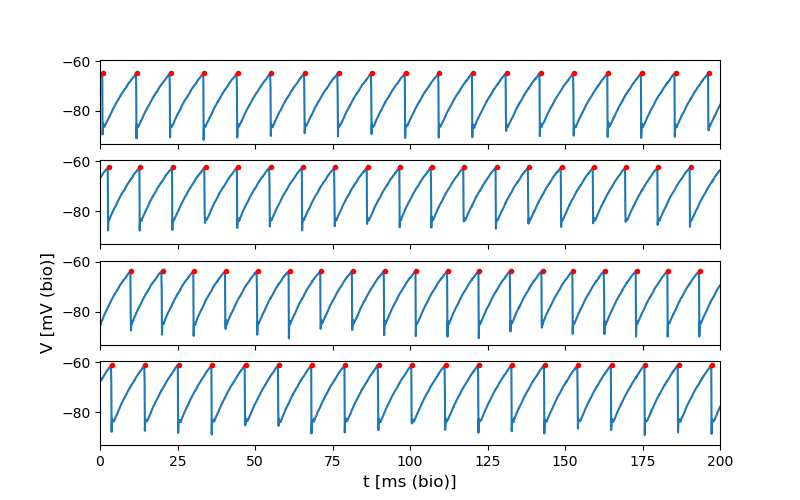
\includegraphics[width=\textwidth]{figures/4membranes-calibrated.png}
        \caption{Calibrated membranes}
    \end{subfigure}
    \caption{(a) Biological membrane potential of four membranes with the same
    setting. The red dots indicate when the digital processing units recognizes
    that voltage reaches the threshold. The rates for the signals are
    \SI{1.02(2)e1}{\milli\second}, \SI{2.41(3)e1}{\milli\second},
    \SI{2.36(1)e1}{\milli\second}, \SI{1.15(1)e1}{\milli\second}, in the same
    order that they presented in the image.
    (b) The same 4 membranes after having been calibrated manually.}
    \label{fig:4membranes}
\end{figure}

The scale of the problem becomes even more clear when considering the that one
half of the SPIKEY chip has a rate distribution like presented in figure
\ref{fig:distribution}, the previous method of trial and error becomes rather
infeasible.

\begin{figure}[ht]
    \centering
    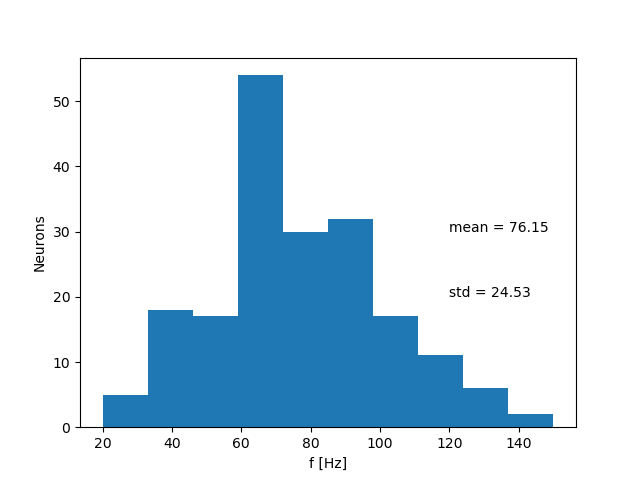
\includegraphics[width=\textwidth]{figures/rate-distribution.png}
    \caption{Distribution of firing rate for the same across one side of the
    chip.}
    \label{fig:distribution}
\end{figure}

Instead an algorithm is suggested that should help find a proper calibration for
all neurons that are able to converge on the desired rate.
\begin{enumerate}
    \item Set the $g_l$ to the default value and measure the rate of the neuron.
    \item Set the $g_l$ to double the default value and measure the rate of the
        neuron.
    \item Describe the response of the neuron linearly using the last two
        points and estimate where the desired rate would lie.
    \item Set the $g_l$ to this value and measure the rate, if it is within the
        standard error: success! If not return to step 3.
\end{enumerate}
Sadly we were unable to implement the algorithm, but we encourage the reader
to.


\subsection{A Single Neuron with Synaptic Input}
Having confirmed that the most basic behaviour of the chip agrees with the
expectations of the model,  a more complicated setup could be investigated.
The computational power of neurons stems from their interconnectedness.  Thus it
is crucial to evaluate how a neuron responds to input from other neurons
(synaptic input).  The quantity of interest here is the membrane potential of
the neuron under scrutiny.  This voltage can be easily monitored as a function
of time using the pynn.record() function.  As discussed in the theory section,
we have two types of synapses: Excitatory ones inducing positive spikes and
inhibitory ones inducing negative spikes.  It is actually crucial to have both
types of synapses to perform calculations.  This can be understood analogously
to positive and negative weights in artificial neural network that describe the
influence of some features on the neuron.  Besides the requirement to have two
different types of synapses that have different behaviour it is also crucial to
examine in what ways the synapse can form the standard input of a spike into
an EPSP.  That is,  how big the transmitted spike will be and how fast it decays.

\subsubsection{.}
To start with the latter,  the effect of the parameters \textbf{drvifall} and
\textbf{drviout} was investigated.  The following results were found:
\begin{itemize}
	\item \textbf{Drviout} controls the magnitude of the voltage spike.  By
	increasing its value the spike height was reduced.
	\item \textbf{Drvifall} controls the width of the peak, that is,  how fast
	it decays.  Increasing this parameter makes the peak more sharp.
\end{itemize}
It could also be observed that those two parameters did not only affect the
height or width of the voltage spike exclusively.  Instead,  decreasing drvifall
was also found to lead to spike of smaller magnitude besides making the
voltage ramp fall more slowly.  This is important to consider since it affects
the degree of precision to which we can fine-tune the EPSP of a neuron.

\begin{figure}[ht]
    \centering
    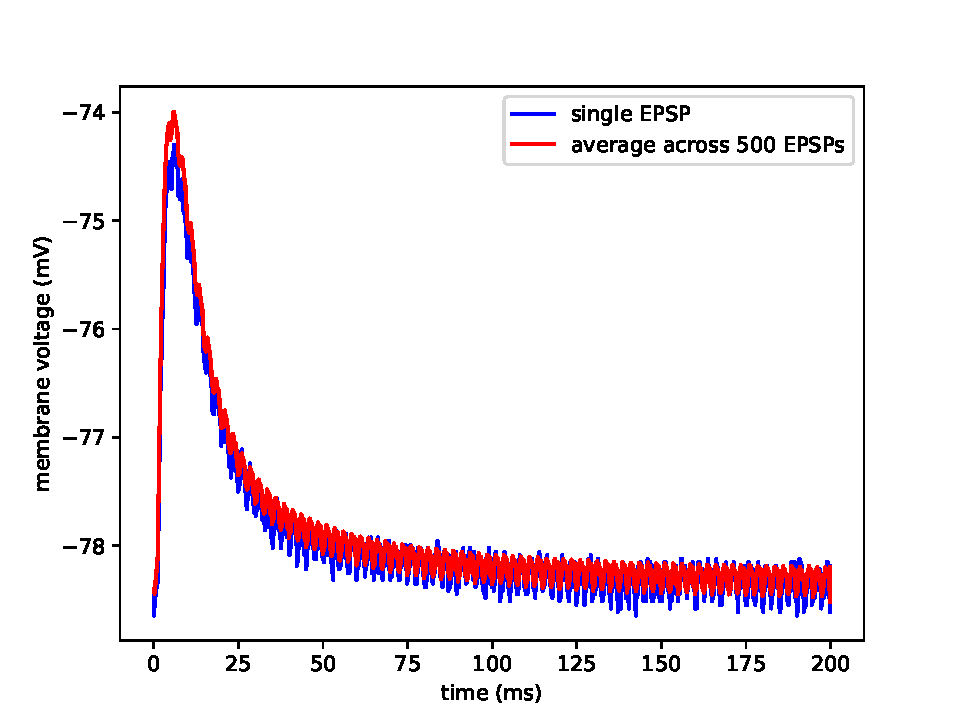
\includegraphics[width=\textwidth]{figures/epsp_default.pdf}
    \caption{Post synaptic potential for default settings of parameters}
    \label{fig:epsp_default}
\end{figure}
\begin{figure}[ht]
    \centering
    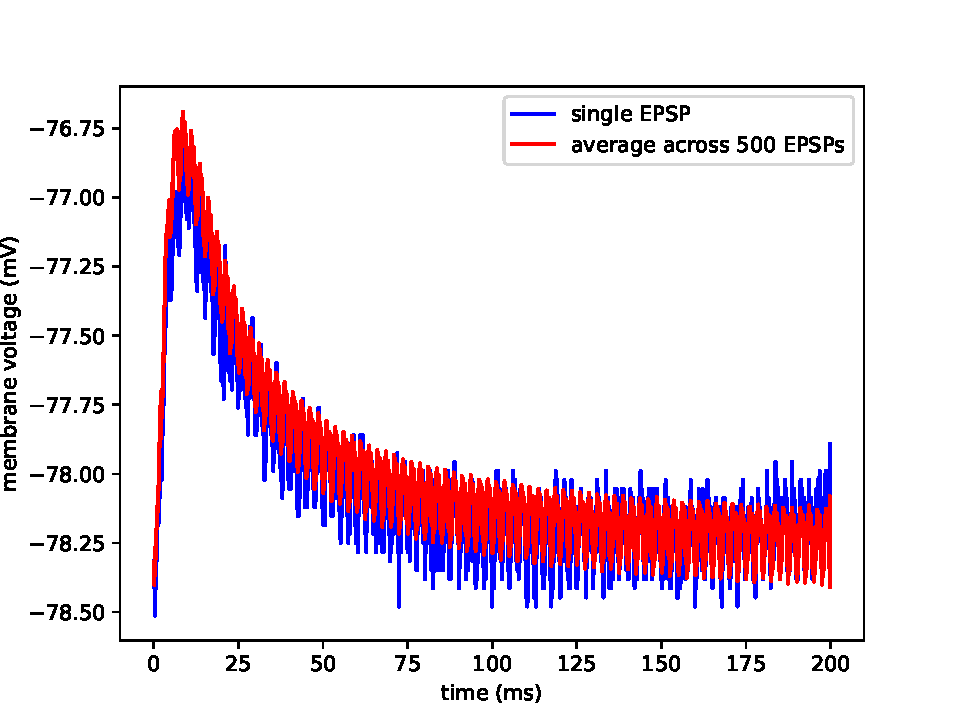
\includegraphics[width=\textwidth]{figures/epsp_out_-.pdf}
    \caption{EPSP for low drviout.}
    \label{fig:epsp_out-}
\end{figure}
\begin{figure}[ht]
    \centering
    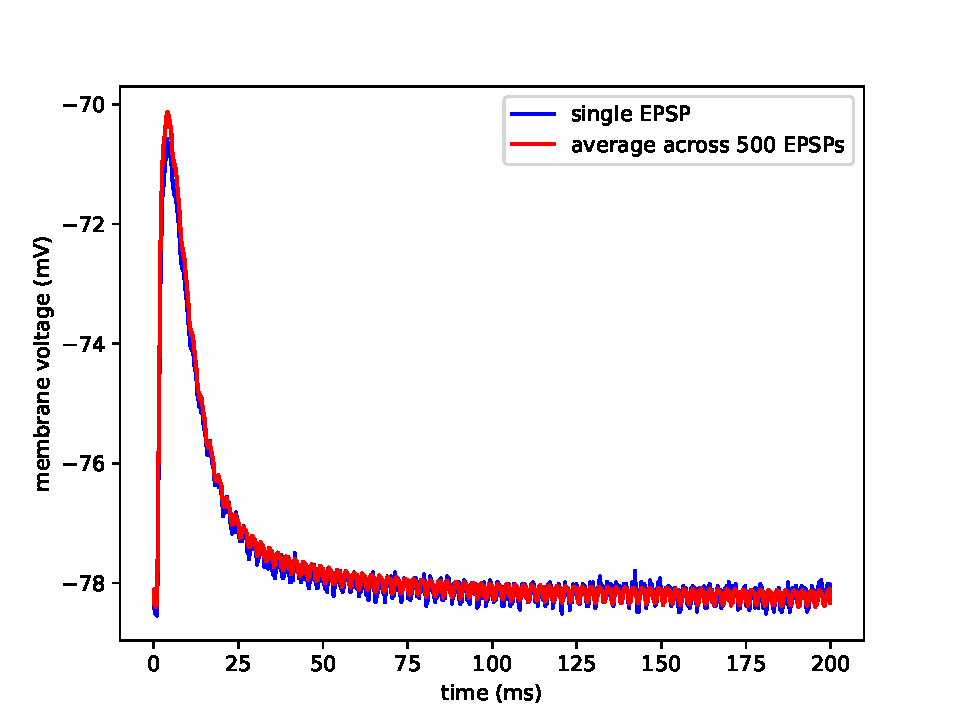
\includegraphics[width=\textwidth]{figures/epsp_out_+.pdf}
    \caption{EPSP for high drviout.}
    \label{fig:epsp_out+}
\end{figure}
\begin{figure}[ht]
    \centering
    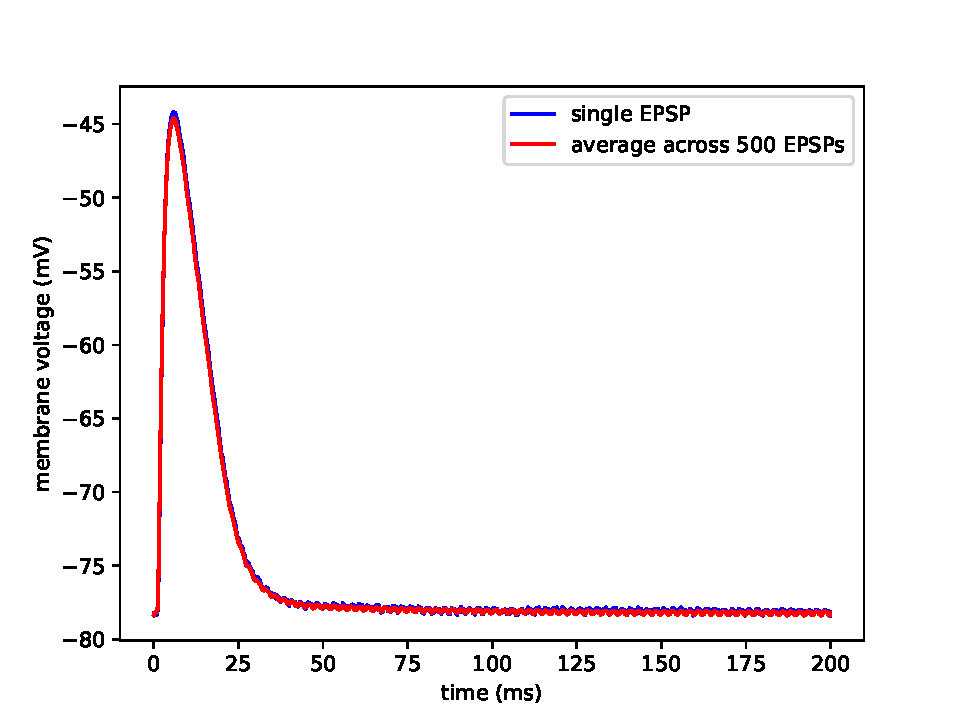
\includegraphics[width=\textwidth]{figures/epsp_fall_-.pdf}
    \caption{EPSP for low drvifall.}
    \label{fig:epsp_fall-}
\end{figure}
\begin{figure}[ht]
    \centering
    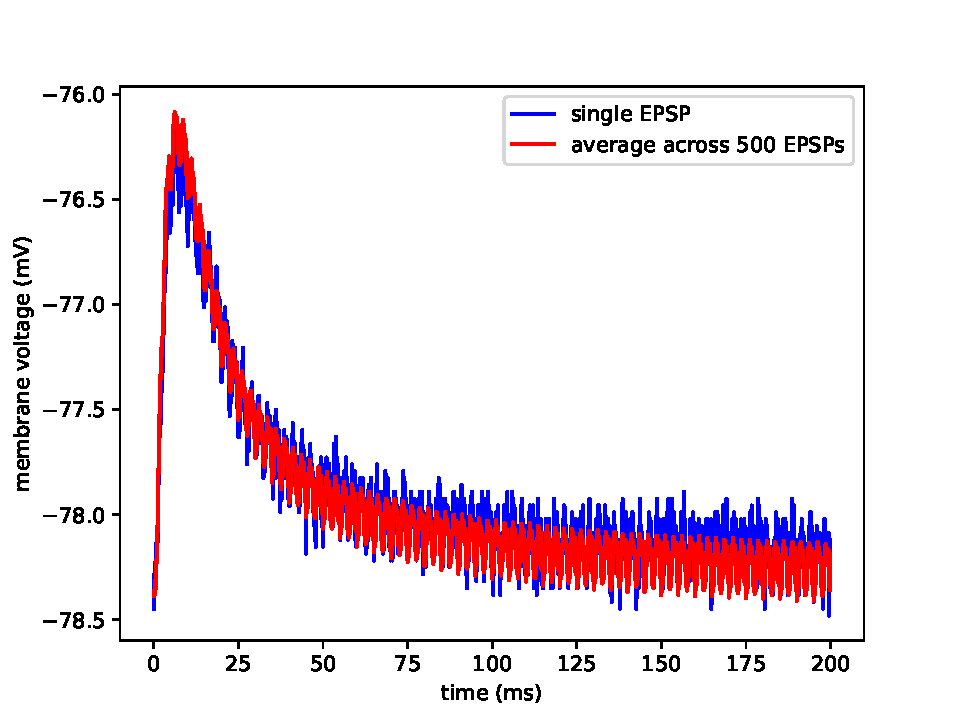
\includegraphics[width=\textwidth]{figures/epsp_fall_+.pdf}
    \caption{EPSP for high drvifall.}
    \label{fig:epsp_fall+}
\end{figure}
\subsubsection{.}
To verify that apart from the shape the general form of the signal could
also be modified,  the parameters were set in such a way that inhibitory
synapses were achieved.  For the same parameters (\textbf{drvifall} = 0.3,
\textbf{drviout} = 0.5) the EPSP was observed for both inhibitory and
excitatory neurons.  It can clearly be seen how they lead to different shapes.
\begin{figure}
    				\centering
    				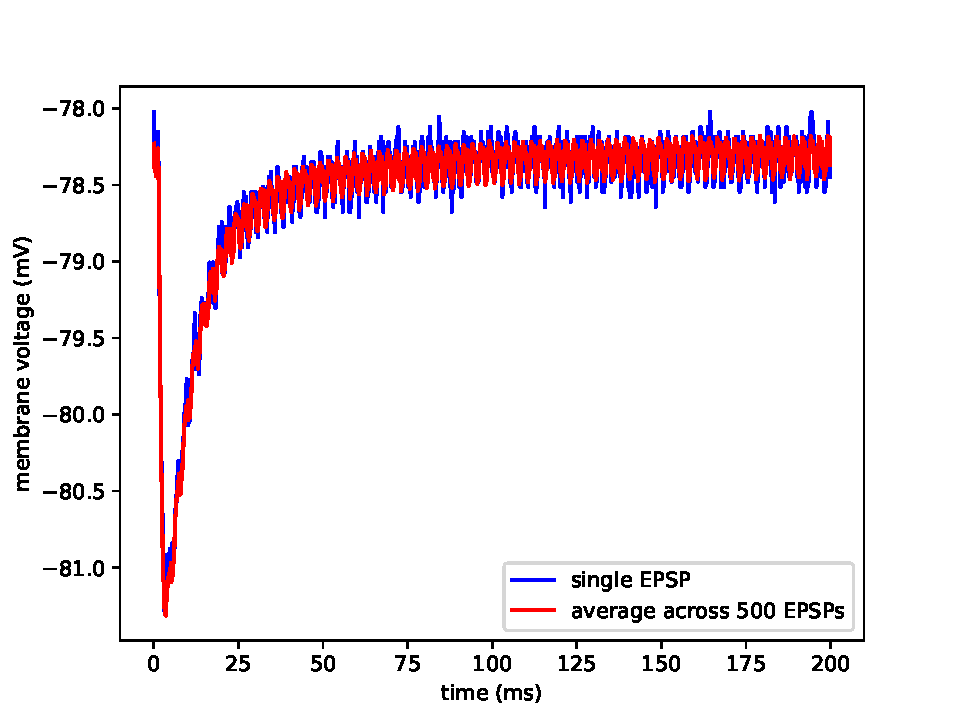
\includegraphics[width=\linewidth]{figures/epsp_inh_fall_03_out_05.pdf}
    				\label{inh_syn}
\end{figure}
  \begin{figure}
    				\centering
    				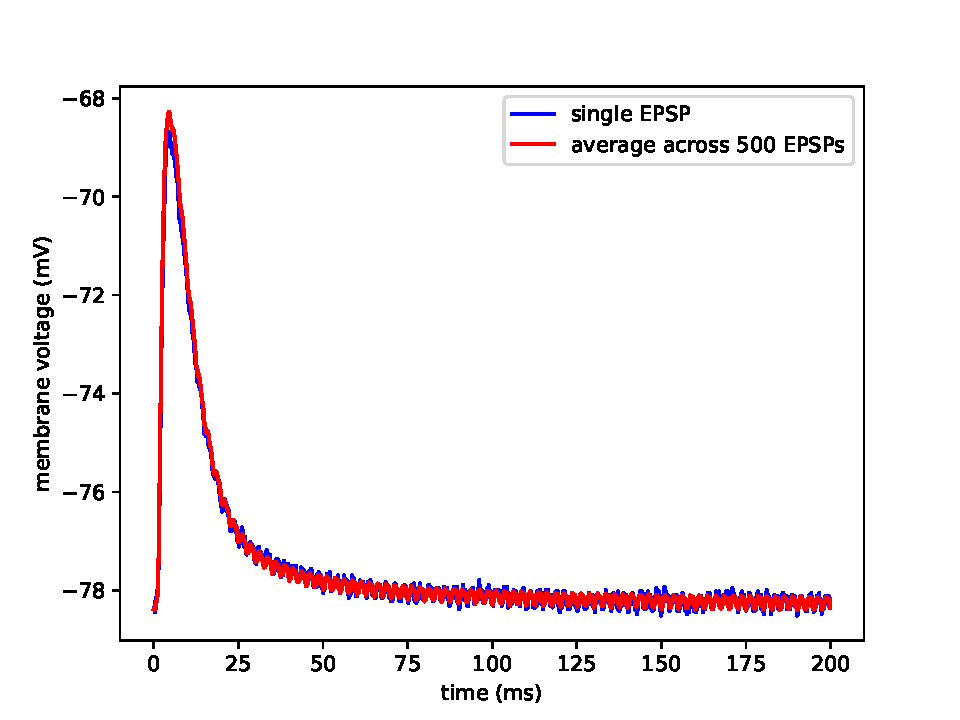
\includegraphics[width=\linewidth]{figures/epsp_exc_fall_03_out_05.pdf}
    				\label{exc_syn}
    				%\caption{source: FP09 neuromorphic computing script,  2020}
\end{figure}
\subsubsection{.}
Besides investigating whether the simple circuits behave as expected, it is also
crucial to develop an idea of what role fluctuations play in this experiment.  Only
if we know the source and extent of fluctuations can we try to work on a model
that corrects them when we want to use the neuromorphic chip for actual
computations.  Before,  we have already looked at temporal noise (e.g. for the
regular spiking regime in ex.1).  Now we want to investigate the synapse-to-synapse
noise.  For this we vary the row of the stimulating synapse for identical
parameters and plot a histogram of the EPSP heights.  In \ref{MaxVoltHisto} this
distribution can be seen.  It is quite obvious that despite identical parameters
the individual stimulating synapse matters a long with regards to the resulting
EPSP height.  The mean is $3.06$mV,  but since the distribution is clearly
asymmetric,  the median is a more meaningful quantity.  This was determined
to be $2.64$.  The standard deviation is with $1.17$mV very large.  We can
conclude that production errors of different synapses need to be taken into
account to get correct results.
\begin{figure}
		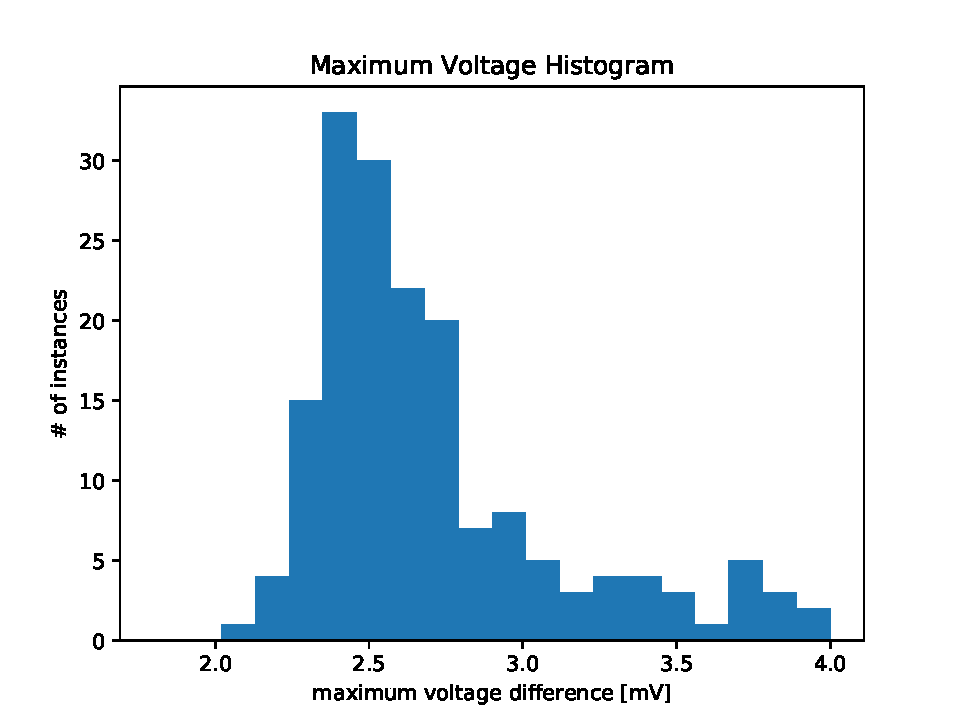
\includegraphics[width=0.7\textwidth]{figures/histo_maxVolt.pdf}
		\label{MaxVoltHisto}
	\end{figure}
\subsection{Short Term Plasticity}

\subsection{Feed-Forward Networks}

\subsection{Recurrent Networks}

\subsection{A Simple Computation - XOR}

\section{Results}

\subsection{Investigating A Single Neuron}

\subsection{Calibrating Neuron Parameters}

\subsection{A Single Neuron with Synaptic Input}

\subsection{Short Term Plasticity}

\subsection{Feed-Forward Networks}
Of particular interest in discussing sensitivity of the network to changes in
the connection weights is the `width' of the signal, that is the amount of
spikes fired by the network in response to a single input.

On the SPIKEY chip the there are 15 distinguishable weights that can be
assigned to a connection. 1 being the lowest possible connection strength and 15
the highest.

It was found that easily underestimated connections are the ex->inh and inh->ex
weights. When these are not activated, it is highly likely that the network will
have a continually increasing width if no inhibition is performed at all (see
figure \ref{fig:ff-expansion}).

\begin{figure}
    \centering
    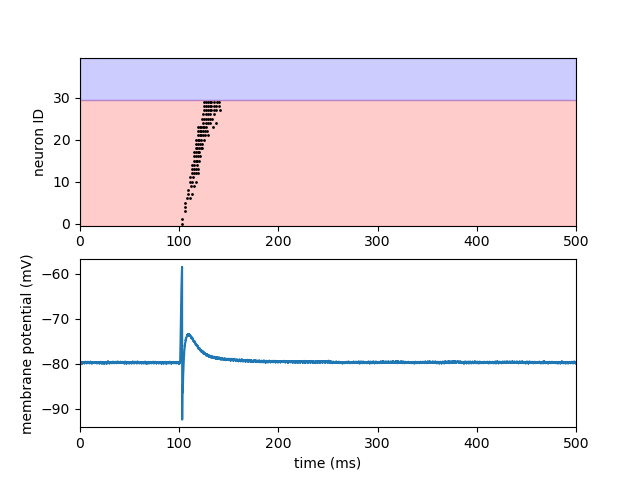
\includegraphics[width=\textwidth]{figures/feedforward-expansion.png}
    \caption{Expansion of the width of a feed forward network when no inhibition
        takes place. Weights used here were: ex0$\rightarrow$ex = 15, ex0 $\rightarrow$ inh = 12, ex $\rightarrow$ ex
        = 15, ex $\rightarrow$ inh = 1, inh $\rightarrow$ ex = 1, in a chain of length 10 and a population
        size of 3 (ex)}
    \label{fig:ff-expansion}
\end{figure}

The longest open chain that was possible to be produced had a length of 48
neurons. This was because the smallest possible population at which a
consistent chain could be created was 3 for excitatory and 1 for the inhibitory
part of the chain. Even when inhibition was set to 1 and the ex $\rightarrow$ ex
connections were set 15, no output was generated when the population size of the
excitatory neurons was 2. Having the population size so low, required the ex
$\rightarrow$ ex connection strength to be near its maximal value (14) to be
able to maintain the signal wave. This in turn meant that the inhibition could
not be set sufficiently high and therefore the signal width keeps increasing as
seen in figure \ref{fig:ff-open-3-1}.

\begin{figure}
    \centering
    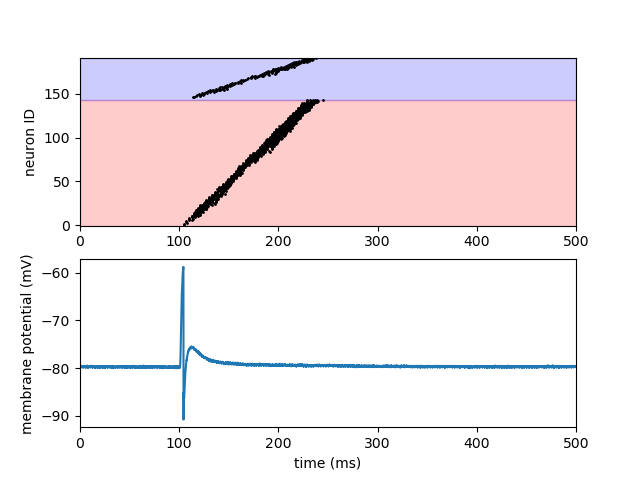
\includegraphics[width=\textwidth]{figures/feedforward-open.png}
    \caption{Open chain at maximal length (48) with population size 3 for
    excitatory neurons and 1 for inhibitory neurons. The weights used were ex0
    $\rightarrow$ ex = 13, ex0 $\rightarrow$ inh = 7, ex $\rightarrow$ ex= 14,
    ex $\rightarrow$ inh = 7, inh $\rightarrow$ ex = 15. The final width lies around
    8.}
    \label{fig:ff-open-3-1}
\end{figure}

In order to combat this effect an extra inhibitory neuron was added, shrinking
the maximum length to 38 neurons, however this allowed for getting a very clean
signal with an average width of only 1.2, as can be seen in figure

\begin{figure}
    \centering
    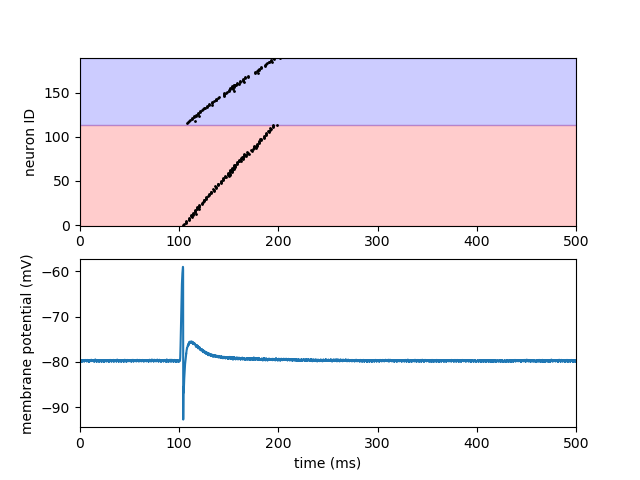
\includegraphics[width=\textwidth]{figures/feedforward-open-better.png}
    \caption{Open chain at maximal length (38) with population size 3 for
    excitatory neurons and 2 for inhibitory neurons. The weights used were
    ex0 $\rightarrow$ ex = 13, ex0 $\rightarrow$ inh = 7, ex $\rightarrow$ ex =
    14, ex $\rightarrow$ inh = 10, inh $\rightarrow$ ex = 15. The final signal width
    was about 2.}
    \label{fig:ff-open-3-2}
\end{figure}

An interesting phenomena occurs when the network is configured to loop, that is
to say the last neuron excites the first. It was not possible to set the
signal delay, which would have allowed for more careful investigation, by being
able to see which signals were caused by an excitatory neuron signaling too
often and what was the next round of signals, but still there was a clear effect
visible in figure \ref{fig:feed-forward-loop}. Note worthy is that this change
of connection required a reconfiguring of the network, which indicates that
creating connections changes the effective weights in the network.

\begin{figure}
    \centering
    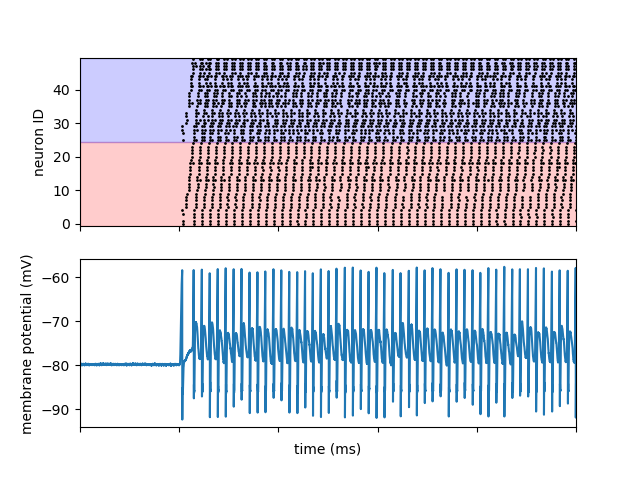
\includegraphics[width=.5\textwidth]{figures/feedforward-signals-loop.png}
    \caption{Open chain at maximal length (38) with population size 3 for
    excitatory neurons and 2 for inhibitory neurons. The weights used were
    ex0 $\rightarrow$ ex = 15, ex0 $\rightarrow$ inh = 7, ex $\rightarrow$ ex =
    14, ex $\rightarrow$ inh = 10, inh $\rightarrow$ ex = 15.}
    \label{fig:feed-forward-loop}
\end{figure}

\subsection{Recurrent Networks}

\subsection{A Simple Computation - XOR}
A challenge that comes with a network like this is to find the correct set of
weights in order for the network to operate as expected. This was achieved by
plotting all signals sent in the same graph, as can be seen in figure
\ref{fig:XOR-output}. This allowed for a speedy diagnosis of the network by
showing what expected signals were missing. An additional script was present
that would match the fired signals to expected time stamps, giving a
quantitative description of the quality of the network. This script would
generate input signals, and perform the XOR operation internally, creating an
internal expectation for when each neuron should fire or not.

\begin{figure}
    \centering
    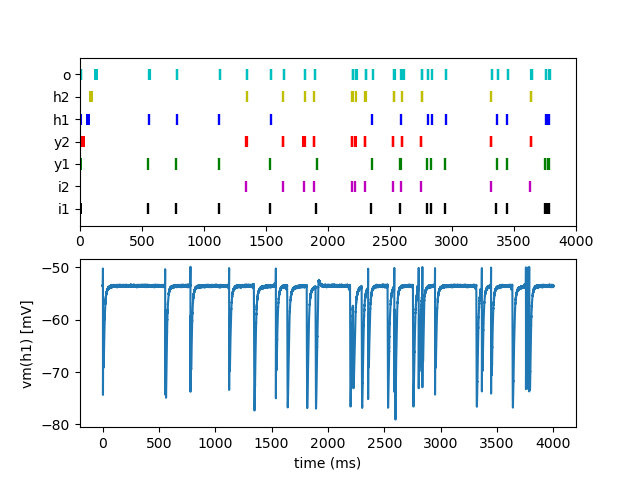
\includegraphics[width=\textwidth]{figures/XOR-output.png}
    \caption{Output of the diagnostic tool for rating the performance of the XOR network.}
    \label{fig:XOR-output}
\end{figure}

It quickly became clear that though a temporarily optimal configuration had been
found, it was not to last long, as a mere half hour later the accuracy had
dropped from 39/40 to 33/40, confirming suspicions from earlier experiments.
However the accuracy was large enough to show that as the input was temporally
shifted using a normal distribution, it did not immediately lose it's accuracy.
Only after the standard deviation of the jitter became larger than 15
milliseconds, network was unable to give a correct output anymore. This is
remarkable fact is likely due to the fact that the potential does not
immediately decay to the rest potential but remains high for some some time.
This could be useful in applications where signals are not perfectly timed, but
relative simultaneity is required.


\section{Final Conclusions}
Our results clearly show that the SPIKEY chip can be used for experimenting with
neuromorphic computing in the physical world. Most importantly, it could
verified that the elementary building block (LIF-circuit) behaved in a very
favourable way. Different characteristic features in different realizations of
that circuit in the hardware (due to production variations) can be observed but it
was shown to be possible to calibrate each  ``neuron'' in a way that the effect
of production errors is mostly cancelled. The circuit allows short term
plasticity,  a key trait of neurons that allows them to `learn'.  Finally,
leaving the few-neuron regime, it was verified that the hardware can be used to
model circuits with $\approx 200$ neurons, even binary logic was achievable with
the hardware.

However thanks to the temporal instability of the chip and its production
variations it is not production ready. It is hard to think of a critical
application that would have environmental conditions suited for this chip, that
would be simultaneously cost effective. Calibration would likely be sufficiently
time consuming that it would ruin any cost effectiveness. That is not to say
that it is without application in the world of research, where it can be a
useful tool to investigate behaviour of neural structures by making it behave
like physical neurons.

\section{Discussion}
Comparing our quite complicated realization of the XOR-gate to the standard
electrical implementation of the binary gate in digital computing leads us to
one final important insight: When switching computer hardware to neuromorphic
hardware, it does not suffice to merely copy the brain's architecture and
continue to use boolean logic like is done in conventional computers. It is far
too fragile, requiring an enormous amount of neurons and an inefficient use of
computation power.

Instead, if neuromorphic computing is to become an integral part of
computational methods, it is key the field adapts to the biological blueprint.
Naturally that would inspire radically new ways of problem solving in signal
processing.

Before that is reached however, a stark increase in the stability of the
hardware is required, as well as an increase in available neurons, as even a
jelly fish has over 5000 neurons \cite{neuronsjellyfish}. This paper has
provided a qualitative review of the chip, however quantitative measurements are
still lacking. We hypothesize that temporal differences in the internal
temperature of the chip is likely the main culprit of this instability,
therefore describing both the sensitivity to a change in temperature and heat
generation by the chip during average usage could be useful indicators of the
chips ability to perform consistently.

\end{document}
